\subsection{Robots on rails}\label{sec::rail}
In industry, HVOF coating processes are performed by robotic manipulators,
which offer tasks versatility and large workspace, required for this
type of application. Meanwhile, a robotic arm capable of coating all the turbine
blade surface on a fixed position is not compact or mobile, and hard to be
mounted/unmounted. A prismatic joint coupled to a rail is a common strategy for
extending the robot working space, without adding weight to the manipulator,
and the rail can use the structures in the environment as a support.
%Na indústria, a automatização de processos de metalização, é
%normalmente realizada com a utilização de manipuladores robóticos, pois oferece
%a versatilidade de tarefas e espaço de trabalho necessários para esse
%tipo de aplicação. Entretanto, um sistema composto por um braço robótico capaz
%de operar em toda a extensão da superfície da pá da turbina hidrelétrica
%não é compacto, nem móvel o suficiente para ser instalado e desinstalado para a
%operação de manuntenção \textit{in-situ}.


%A introdução de uma junta prismática acoplada a um trilho é uma estratégia para
%reduzir o tamanho e o peso de um manipulador robótico.  Assim, é possível
% estender o espaço de trabalho do robô, sem adicionar peso ao manipulador, uma vez que o
% trilho pode usar as estruturas presentes no ambiente como apoio. 


%Na literatura foram encontradas duas soluções para aplicações de manutenção e
%inspeção, como solda, específicas para o contexto de turbinas hidráulicas. As
%aplicações diferem, principalmente, na estratégia de fixação do sistema
%de trilhos.
%O Roboturb \citep{roboturb} realiza a fixação
%diretamente na pá do rotor, enquanto o robô Scompi \citep{scompi} utiliza um
% trilho fixado em
%estruturas adjacentes à pá ou peça a ser reparada.

The Roboturb \citep{roboturb} is a robotic manipulator composed of six
revolution joints and one prismatic joint coupled to a flexible rail.
%figure~\ref{fig::roboturb}. 
The robot performs welding, filling cavities generated by erosion. The rail
may be shaped and then fixed to the blade surface by a passive system of
suction cups. The robot has two end-effectors: an optical sensor for erosion
inspection; and a welding tool, a PWH-4A plasma torch with automatic feeder.
%O Roborturb \citep{roboturb} consiste em um manipulador robótico com seis
% juntas de revolução e uma junta primsática acoplada a um trilho flexível, como pode ser observado
%na figura \ref{fig::roboturb}, utilizado para o preenchimento de cavidades
%geradas por cavitação.
%O trilho pode ser conformado e, então, fixado à superfície da pá por meio de um
%sistema passivo de ventosas ou ímãs. O robô tem a possibilidade de utilizar
% dois efetuadores distintos, o primeiro consiste em um sensor ótico para inspeção do 
%estado de erosão da pá e o segundo consiste em uma ferramenta de solda do 
%tipo tocha plasma PWH-4A com alimentador automático de arame, responsável pelo 
%depósito de solda para o preenchimento das cavidades identificadas pelo
% sistema.


%TODO Abelha: Posicionar corretamente as figuras
%    \begin{figure}[h!]	
%		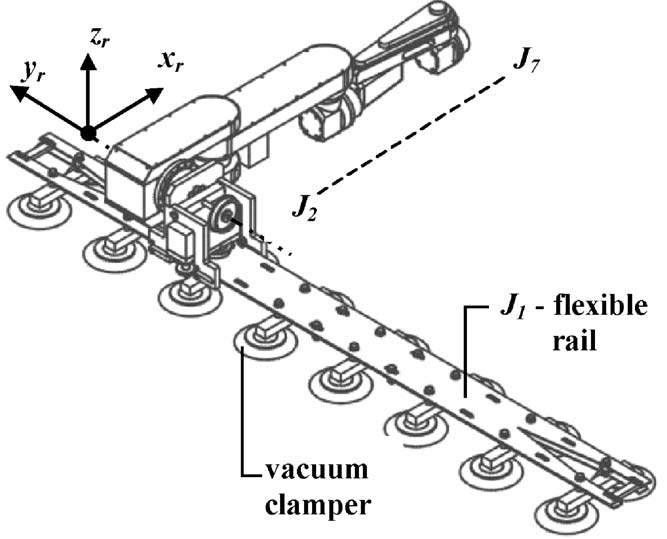
\includegraphics[width=\columnwidth]{figs/trilhos/roboturbpaper}
%		\caption{Roboturb - Robotic manipulator on rail}
%		\label{fig::roboturb}
%	\end{figure}
%	\begin{figure}[h!]
%		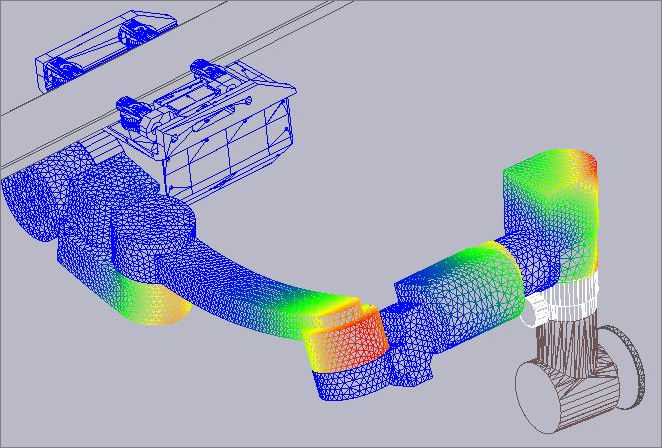
\includegraphics[width=\columnwidth]{figs/trilhos/scompi}
%		\caption{SCOMPI - Manipulador robótico sobre trilhos rígidos}
%		\label{fig::scompi}
%	\end{figure}

The Scompi robot \citep{scompi}%, figure~\ref{fig::scompi}, 
is a multipurpose manipulator, designed to perform repairs on \textit{Francis}
type turbines, as welding and grinding. It has six degrees of freedom: a robotic
manipulator with five revolution joints; and a prismatic joint, coupled to
curved rails that are designed specifically for each application.
%Por sua vez, o robô Scompi \citep{scompi}, fig \ref{fig::scompi}, é um
%manipulador multipropósito projetado para realizar reparos em turbinas do tipo
% \textit{Francis}, como solda e esmerilhamento das pás. O sistema possui seis graus de liberdade,
%sendo consitituído por um braço robótico com cinco juntas de revolução, e o
%último grau de liberdade proveniente de uma junta prismática que percorre um
% sistema de trilhos retos ou curvos que são projetados para cada aplicação especificamente. 


%Sistemas baseados em trilhos tem como maior benefício a redução do tamanho e,
%consequentemente, do peso do manipulador necessário para a execução de tarefas
%em um espaço de trabalho que englobe toda a superfície da pá.
%Essa redução proporciona facilidade de transporte do robô até o interior da
%turbina e também possibilita o projeto de manipuladores que tenham a rigidez
%necessária para a realização das tarefas desejadas. 

Fixed robotic manipulators which meets the HVOF payload and
workspace requirements would be too heavy. Systems based on rails fixed
on the blade itself, require rail handling as the entire
blade surface should be coated and the area in which the rail is fixed is not in
the robot workspace. In addition, rail systems fixed on adjacent structures
should considerate the installation conditions and balance the cost-benefit
of installation/removal rail, and robustness.
%Manipuladores robótico fixos, rígidos o suficiente para aguentar as forças
% intrínsecas ao processo de metalização e com espaço de trabalho necessário para trabalhar em
%toda a extensão da superfćie da pá seriam muito pesados.
%Entretanto, sistemas baseados em trilhos com fixação na própria pá do rotor,
% necessitam que o trilho seja movido caso se deseje que toda a superfície da pá sofra
%manuntenção, uma vez que a área em que o trilho está apoiado não pertence ao
% espaço de trabalho do robô. Em adição, sistemas com fixação de trilhos nas estruturas
%adjacentes à pá devem atentar as condições para a instalação disposta pelo
%ambiente para equilibrar a relação de custo benefício entre facilidade de
%instalação/remoção do trilho e a robustez.
The system advantages are: 1) manipulator size reduction; 2) manipulator
weight reduction. The disadvantages are: 1) rail mounting and unmouting; 2) rail
handling if fixed on the blade.